% Created by tikzDevice version 0.12 on 2019-05-20 04:28:21
% !TEX encoding = UTF-8 Unicode
\begin{tikzpicture}[x=1pt,y=1pt]
\definecolor{fillColor}{RGB}{255,255,255}
\path[use as bounding box,fill=fillColor,fill opacity=0.00] (0,0) rectangle (252.94,252.94);
\begin{scope}
\path[clip] ( 49.20, 61.20) rectangle (227.75,203.75);
\definecolor{drawColor}{RGB}{0,0,0}

\path[draw=drawColor,line width= 0.4pt,line join=round,line cap=round] (138.47,132.47) circle (  2.25);
\end{scope}
\begin{scope}
\path[clip] (  0.00,  0.00) rectangle (252.94,252.94);
\definecolor{drawColor}{RGB}{0,0,0}

\path[draw=drawColor,line width= 0.4pt,line join=round,line cap=round] ( 55.81, 61.20) -- (221.13, 61.20);

\path[draw=drawColor,line width= 0.4pt,line join=round,line cap=round] ( 55.81, 61.20) -- ( 55.81, 55.20);

\path[draw=drawColor,line width= 0.4pt,line join=round,line cap=round] ( 97.14, 61.20) -- ( 97.14, 55.20);

\path[draw=drawColor,line width= 0.4pt,line join=round,line cap=round] (138.47, 61.20) -- (138.47, 55.20);

\path[draw=drawColor,line width= 0.4pt,line join=round,line cap=round] (179.80, 61.20) -- (179.80, 55.20);

\path[draw=drawColor,line width= 0.4pt,line join=round,line cap=round] (221.13, 61.20) -- (221.13, 55.20);

\node[text=drawColor,anchor=base,inner sep=0pt, outer sep=0pt, scale=  1.00] at ( 55.81, 39.60) {0.6};

\node[text=drawColor,anchor=base,inner sep=0pt, outer sep=0pt, scale=  1.00] at ( 97.14, 39.60) {0.8};

\node[text=drawColor,anchor=base,inner sep=0pt, outer sep=0pt, scale=  1.00] at (138.47, 39.60) {1.0};

\node[text=drawColor,anchor=base,inner sep=0pt, outer sep=0pt, scale=  1.00] at (179.80, 39.60) {1.2};

\node[text=drawColor,anchor=base,inner sep=0pt, outer sep=0pt, scale=  1.00] at (221.13, 39.60) {1.4};

\path[draw=drawColor,line width= 0.4pt,line join=round,line cap=round] ( 49.20, 66.48) -- ( 49.20,198.47);

\path[draw=drawColor,line width= 0.4pt,line join=round,line cap=round] ( 49.20, 66.48) -- ( 43.20, 66.48);

\path[draw=drawColor,line width= 0.4pt,line join=round,line cap=round] ( 49.20, 99.48) -- ( 43.20, 99.48);

\path[draw=drawColor,line width= 0.4pt,line join=round,line cap=round] ( 49.20,132.47) -- ( 43.20,132.47);

\path[draw=drawColor,line width= 0.4pt,line join=round,line cap=round] ( 49.20,165.47) -- ( 43.20,165.47);

\path[draw=drawColor,line width= 0.4pt,line join=round,line cap=round] ( 49.20,198.47) -- ( 43.20,198.47);

\node[text=drawColor,rotate= 90.00,anchor=base,inner sep=0pt, outer sep=0pt, scale=  1.00] at ( 34.80, 66.48) {0.6};

\node[text=drawColor,rotate= 90.00,anchor=base,inner sep=0pt, outer sep=0pt, scale=  1.00] at ( 34.80, 99.48) {0.8};

\node[text=drawColor,rotate= 90.00,anchor=base,inner sep=0pt, outer sep=0pt, scale=  1.00] at ( 34.80,132.47) {1.0};

\node[text=drawColor,rotate= 90.00,anchor=base,inner sep=0pt, outer sep=0pt, scale=  1.00] at ( 34.80,165.47) {1.2};

\node[text=drawColor,rotate= 90.00,anchor=base,inner sep=0pt, outer sep=0pt, scale=  1.00] at ( 34.80,198.47) {1.4};

\path[draw=drawColor,line width= 0.4pt,line join=round,line cap=round] ( 49.20, 61.20) --
	(227.75, 61.20) --
	(227.75,203.75) --
	( 49.20,203.75) --
	( 49.20, 61.20);
\end{scope}
\begin{scope}
\path[clip] (  0.00,  0.00) rectangle (252.94,252.94);
\definecolor{drawColor}{RGB}{0,0,0}

\node[text=drawColor,anchor=base,inner sep=0pt, outer sep=0pt, scale=  1.20] at (138.47,224.20) {\bfseries Hello World!};

\node[text=drawColor,anchor=base,inner sep=0pt, outer sep=0pt, scale=  1.00] at (138.47, 15.60) {Index};

\node[text=drawColor,rotate= 90.00,anchor=base,inner sep=0pt, outer sep=0pt, scale=  1.00] at ( 10.80,132.47) {1};
\end{scope}
\end{tikzpicture}
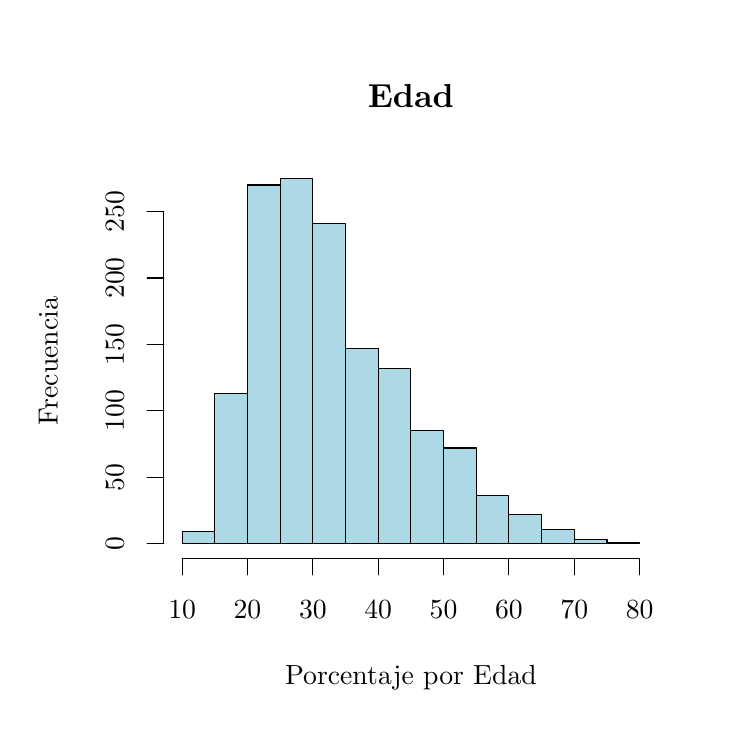
\begin{tikzpicture}[x=1pt,y=1pt]
\definecolor{fillColor}{RGB}{255,255,255}
\path[use as bounding box,fill=fillColor,fill opacity=0.00] (0,0) rectangle (252.94,252.94);
\begin{scope}
\path[clip] (  0.00,  0.00) rectangle (252.94,252.94);
\definecolor{drawColor}{RGB}{0,0,0}

\node[text=drawColor,anchor=base,inner sep=0pt, outer sep=0pt, scale=  1.20] at (138.47,224.20) {\bfseries Edad};

\node[text=drawColor,anchor=base,inner sep=0pt, outer sep=0pt, scale=  1.00] at (138.47, 15.60) {Porcentaje por Edad};

\node[text=drawColor,rotate= 90.00,anchor=base,inner sep=0pt, outer sep=0pt, scale=  1.00] at ( 10.80,132.47) {Frecuencia};
\end{scope}
\begin{scope}
\path[clip] (  0.00,  0.00) rectangle (252.94,252.94);
\definecolor{drawColor}{RGB}{0,0,0}

\path[draw=drawColor,line width= 0.4pt,line join=round,line cap=round] ( 55.81, 61.20) -- (221.13, 61.20);

\path[draw=drawColor,line width= 0.4pt,line join=round,line cap=round] ( 55.81, 61.20) -- ( 55.81, 55.20);

\path[draw=drawColor,line width= 0.4pt,line join=round,line cap=round] ( 79.43, 61.20) -- ( 79.43, 55.20);

\path[draw=drawColor,line width= 0.4pt,line join=round,line cap=round] (103.05, 61.20) -- (103.05, 55.20);

\path[draw=drawColor,line width= 0.4pt,line join=round,line cap=round] (126.66, 61.20) -- (126.66, 55.20);

\path[draw=drawColor,line width= 0.4pt,line join=round,line cap=round] (150.28, 61.20) -- (150.28, 55.20);

\path[draw=drawColor,line width= 0.4pt,line join=round,line cap=round] (173.90, 61.20) -- (173.90, 55.20);

\path[draw=drawColor,line width= 0.4pt,line join=round,line cap=round] (197.52, 61.20) -- (197.52, 55.20);

\path[draw=drawColor,line width= 0.4pt,line join=round,line cap=round] (221.13, 61.20) -- (221.13, 55.20);

\node[text=drawColor,anchor=base,inner sep=0pt, outer sep=0pt, scale=  1.00] at ( 55.81, 39.60) {10};

\node[text=drawColor,anchor=base,inner sep=0pt, outer sep=0pt, scale=  1.00] at ( 79.43, 39.60) {20};

\node[text=drawColor,anchor=base,inner sep=0pt, outer sep=0pt, scale=  1.00] at (103.05, 39.60) {30};

\node[text=drawColor,anchor=base,inner sep=0pt, outer sep=0pt, scale=  1.00] at (126.66, 39.60) {40};

\node[text=drawColor,anchor=base,inner sep=0pt, outer sep=0pt, scale=  1.00] at (150.28, 39.60) {50};

\node[text=drawColor,anchor=base,inner sep=0pt, outer sep=0pt, scale=  1.00] at (173.90, 39.60) {60};

\node[text=drawColor,anchor=base,inner sep=0pt, outer sep=0pt, scale=  1.00] at (197.52, 39.60) {70};

\node[text=drawColor,anchor=base,inner sep=0pt, outer sep=0pt, scale=  1.00] at (221.13, 39.60) {80};

\path[draw=drawColor,line width= 0.4pt,line join=round,line cap=round] ( 49.20, 66.48) -- ( 49.20,186.47);

\path[draw=drawColor,line width= 0.4pt,line join=round,line cap=round] ( 49.20, 66.48) -- ( 43.20, 66.48);

\path[draw=drawColor,line width= 0.4pt,line join=round,line cap=round] ( 49.20, 90.48) -- ( 43.20, 90.48);

\path[draw=drawColor,line width= 0.4pt,line join=round,line cap=round] ( 49.20,114.47) -- ( 43.20,114.47);

\path[draw=drawColor,line width= 0.4pt,line join=round,line cap=round] ( 49.20,138.47) -- ( 43.20,138.47);

\path[draw=drawColor,line width= 0.4pt,line join=round,line cap=round] ( 49.20,162.47) -- ( 43.20,162.47);

\path[draw=drawColor,line width= 0.4pt,line join=round,line cap=round] ( 49.20,186.47) -- ( 43.20,186.47);

\node[text=drawColor,rotate= 90.00,anchor=base,inner sep=0pt, outer sep=0pt, scale=  1.00] at ( 34.80, 66.48) {0};

\node[text=drawColor,rotate= 90.00,anchor=base,inner sep=0pt, outer sep=0pt, scale=  1.00] at ( 34.80, 90.48) {50};

\node[text=drawColor,rotate= 90.00,anchor=base,inner sep=0pt, outer sep=0pt, scale=  1.00] at ( 34.80,114.47) {100};

\node[text=drawColor,rotate= 90.00,anchor=base,inner sep=0pt, outer sep=0pt, scale=  1.00] at ( 34.80,138.47) {150};

\node[text=drawColor,rotate= 90.00,anchor=base,inner sep=0pt, outer sep=0pt, scale=  1.00] at ( 34.80,162.47) {200};

\node[text=drawColor,rotate= 90.00,anchor=base,inner sep=0pt, outer sep=0pt, scale=  1.00] at ( 34.80,186.47) {250};
\end{scope}
\begin{scope}
\path[clip] ( 49.20, 61.20) rectangle (227.75,203.75);
\definecolor{drawColor}{RGB}{0,0,0}
\definecolor{fillColor}{RGB}{173,216,230}

\path[draw=drawColor,line width= 0.4pt,line join=round,line cap=round,fill=fillColor] ( 55.81, 66.48) rectangle ( 67.62, 70.80);

\path[draw=drawColor,line width= 0.4pt,line join=round,line cap=round,fill=fillColor] ( 67.62, 66.48) rectangle ( 79.43,120.71);

\path[draw=drawColor,line width= 0.4pt,line join=round,line cap=round,fill=fillColor] ( 79.43, 66.48) rectangle ( 91.24,196.07);

\path[draw=drawColor,line width= 0.4pt,line join=round,line cap=round,fill=fillColor] ( 91.24, 66.48) rectangle (103.05,198.47);

\path[draw=drawColor,line width= 0.4pt,line join=round,line cap=round,fill=fillColor] (103.05, 66.48) rectangle (114.86,182.15);

\path[draw=drawColor,line width= 0.4pt,line join=round,line cap=round,fill=fillColor] (114.86, 66.48) rectangle (126.66,137.03);

\path[draw=drawColor,line width= 0.4pt,line join=round,line cap=round,fill=fillColor] (126.66, 66.48) rectangle (138.47,129.83);

\path[draw=drawColor,line width= 0.4pt,line join=round,line cap=round,fill=fillColor] (138.47, 66.48) rectangle (150.28,107.28);

\path[draw=drawColor,line width= 0.4pt,line join=round,line cap=round,fill=fillColor] (150.28, 66.48) rectangle (162.09,101.04);

\path[draw=drawColor,line width= 0.4pt,line join=round,line cap=round,fill=fillColor] (162.09, 66.48) rectangle (173.90, 83.76);

\path[draw=drawColor,line width= 0.4pt,line join=round,line cap=round,fill=fillColor] (173.90, 66.48) rectangle (185.71, 77.04);

\path[draw=drawColor,line width= 0.4pt,line join=round,line cap=round,fill=fillColor] (185.71, 66.48) rectangle (197.52, 71.76);

\path[draw=drawColor,line width= 0.4pt,line join=round,line cap=round,fill=fillColor] (197.52, 66.48) rectangle (209.32, 67.92);

\path[draw=drawColor,line width= 0.4pt,line join=round,line cap=round,fill=fillColor] (209.32, 66.48) rectangle (221.13, 66.96);
\end{scope}
\end{tikzpicture}
